% Task 6 — Gateway Hub Design
% Northeast Megaregion Freight Network Design
% All throughput figures in thousand short tons (ktons); capacity in square feet (sf); distances in miles.

\section{Task 6 — Gateway Hub Design}

Task~6 operates below the regional hub tier: it partitions each of the 50 Task~3 regions
into smaller freight \emph{areas}, then selects a set of gateway hubs from the CoStar
candidate pool to serve each area. The design proceeds in two phases. Phase~1 clusters
the 434 NE counties into 132 areas via a population-typed Simulated Annealing (SA)
algorithm. Phase~2 selects 312 gateway hubs using a global set-cover MIP analogous in
structure to Task~5 but calibrated for the area tier.

\subsection{Phase 1 — Area Clustering}

\subsubsection{Region Type Classification}

The number of gateway areas within each region is governed by population density. A
composite score $\text{score}_r = 0.6 \cdot \text{rank}(\text{total\_pop}_r) +
0.4 \cdot \text{rank}(\text{max\_county\_pop}_r)$ is computed for each region and
divided into tertiles:

\begin{itemize}
  \item \textbf{Type A (Urban/Metro)} — 17 regions; total population range
        1.25M--8.56M; minimum 4 areas per region.
  \item \textbf{Type B (Suburban)} — 16 regions; total population range
        696k--1.76M; minimum 3 areas per region.
  \item \textbf{Type C (Rural/Sparse)} — 17 regions; total population range
        429k--873k; minimum 2 areas per region.
\end{itemize}

A critical cap rule is applied: no region can be divided into more areas than it has
counties. Applying this cap to the 50-region partition (where 15 regions have fewer than
4 counties) reduces the planned area total from 150 to an effective \textbf{132 areas}:
55 Type~A, 43 Type~B, and 34 Type~C.

\subsubsection{SA Objective and Algorithm}

The area clustering SA minimises a two-component objective within each region
independently:

\begin{equation}
  J_r = w_{\text{compact}} \cdot C_{\text{compact}} + w_{\text{spread}} \cdot C_{\text{spread}}
  \label{eq:task6-obj}
\end{equation}

\begin{align}
  C_{\text{compact}} &= \frac{1}{N_r \cdot D_r^2}
    \sum_{i \in r} \bigl\|(x_i, y_i) - \mu_{a_i}\bigr\|^2
  \label{eq:task6-compact} \\[6pt]
  C_{\text{spread}} &= \frac{1}{k_r} \sum_{a \notin \text{exempt}}
    \left(\frac{\max(0,\; d_{\max,a} - 80\;\text{mi})}{80\;\text{mi}}\right)^2
  \label{eq:task6-spread}
\end{align}

where $D_r$ is the bounding-box diagonal of region $r$; $\mu_{a_i}$ is the unweighted
centroid of area $a_i$; and $d_{\max,a}$ is the maximum pairwise county-centroid distance
within area $a$. Weights are $w_{\text{compact}} = 1.0$ and $w_{\text{spread}} = 2.0$.

Demand balance is intentionally excluded from the objective. Gateway areas are
geographic groupings for hub siting; the Phase~2 MIP scales the number of selected
gateways to each area's freight demand independently. A balance penalty would
unnecessarily constrain the compactness and spread optimisation that determines
cross-area travel times.

Nine large-span regions (span $> 150$~miles: regions 4, 9, 15, 19, 21, 32, 33, 41, 46)
are designated \emph{exempt} from the spread penalty, acknowledging that their geography
cannot satisfy an 80-mile cross-area constraint without fragmenting them beyond the county
count limit.

\paragraph{Hard constraints.}
Each SA move (county $i$ from area $a_{\text{from}}$ to area $a_{\text{to}}$) is accepted
only if: (1) county $i$ is adjacent to area $a_{\text{to}}$; (2) the donor area retains
at least one county; and (3) $a_{\text{from}} \setminus \{i\}$ remains connected
(verified by BFS). The schedule uses $\alpha = 0.998$, $T_0$ sampled empirically, and
2 restarts per region, with $n_{\text{proposals}} = \max(5{,}000,\; 800 \times n_{\text{counties},r})$.

\subsubsection{Area Clustering Results}

The SA produces \textbf{132 contiguous areas} across all 50 regions with zero distance
violations in non-exempt regions (maximum cross-area distance 140.5~miles occurs only
in an exempt large-span region). Table~\ref{tab:task6-areas} summarises the area
partition by region type.

\begin{table}[H]
  \centering
  \caption{Area partition summary by region type.}
  \label{tab:task6-areas}
  \begin{tabular}{lrrr}
    \toprule
    Region type & Regions & Areas & Mean counties/area \\
    \midrule
    A (Urban/Metro)  & 17 & 55 & 3.3 \\
    B (Suburban)     & 16 & 43 & 3.1 \\
    C (Rural/Sparse) & 17 & 34 & 3.4 \\
    \midrule
    \textbf{Total}   & \textbf{50} & \textbf{132} & \textbf{3.3} \\
    \bottomrule
  \end{tabular}
\end{table}

Figure~\ref{fig:task6-areas} maps the 132 areas with region-type labels overlaid.

\begin{figure}[H]
  \centering
  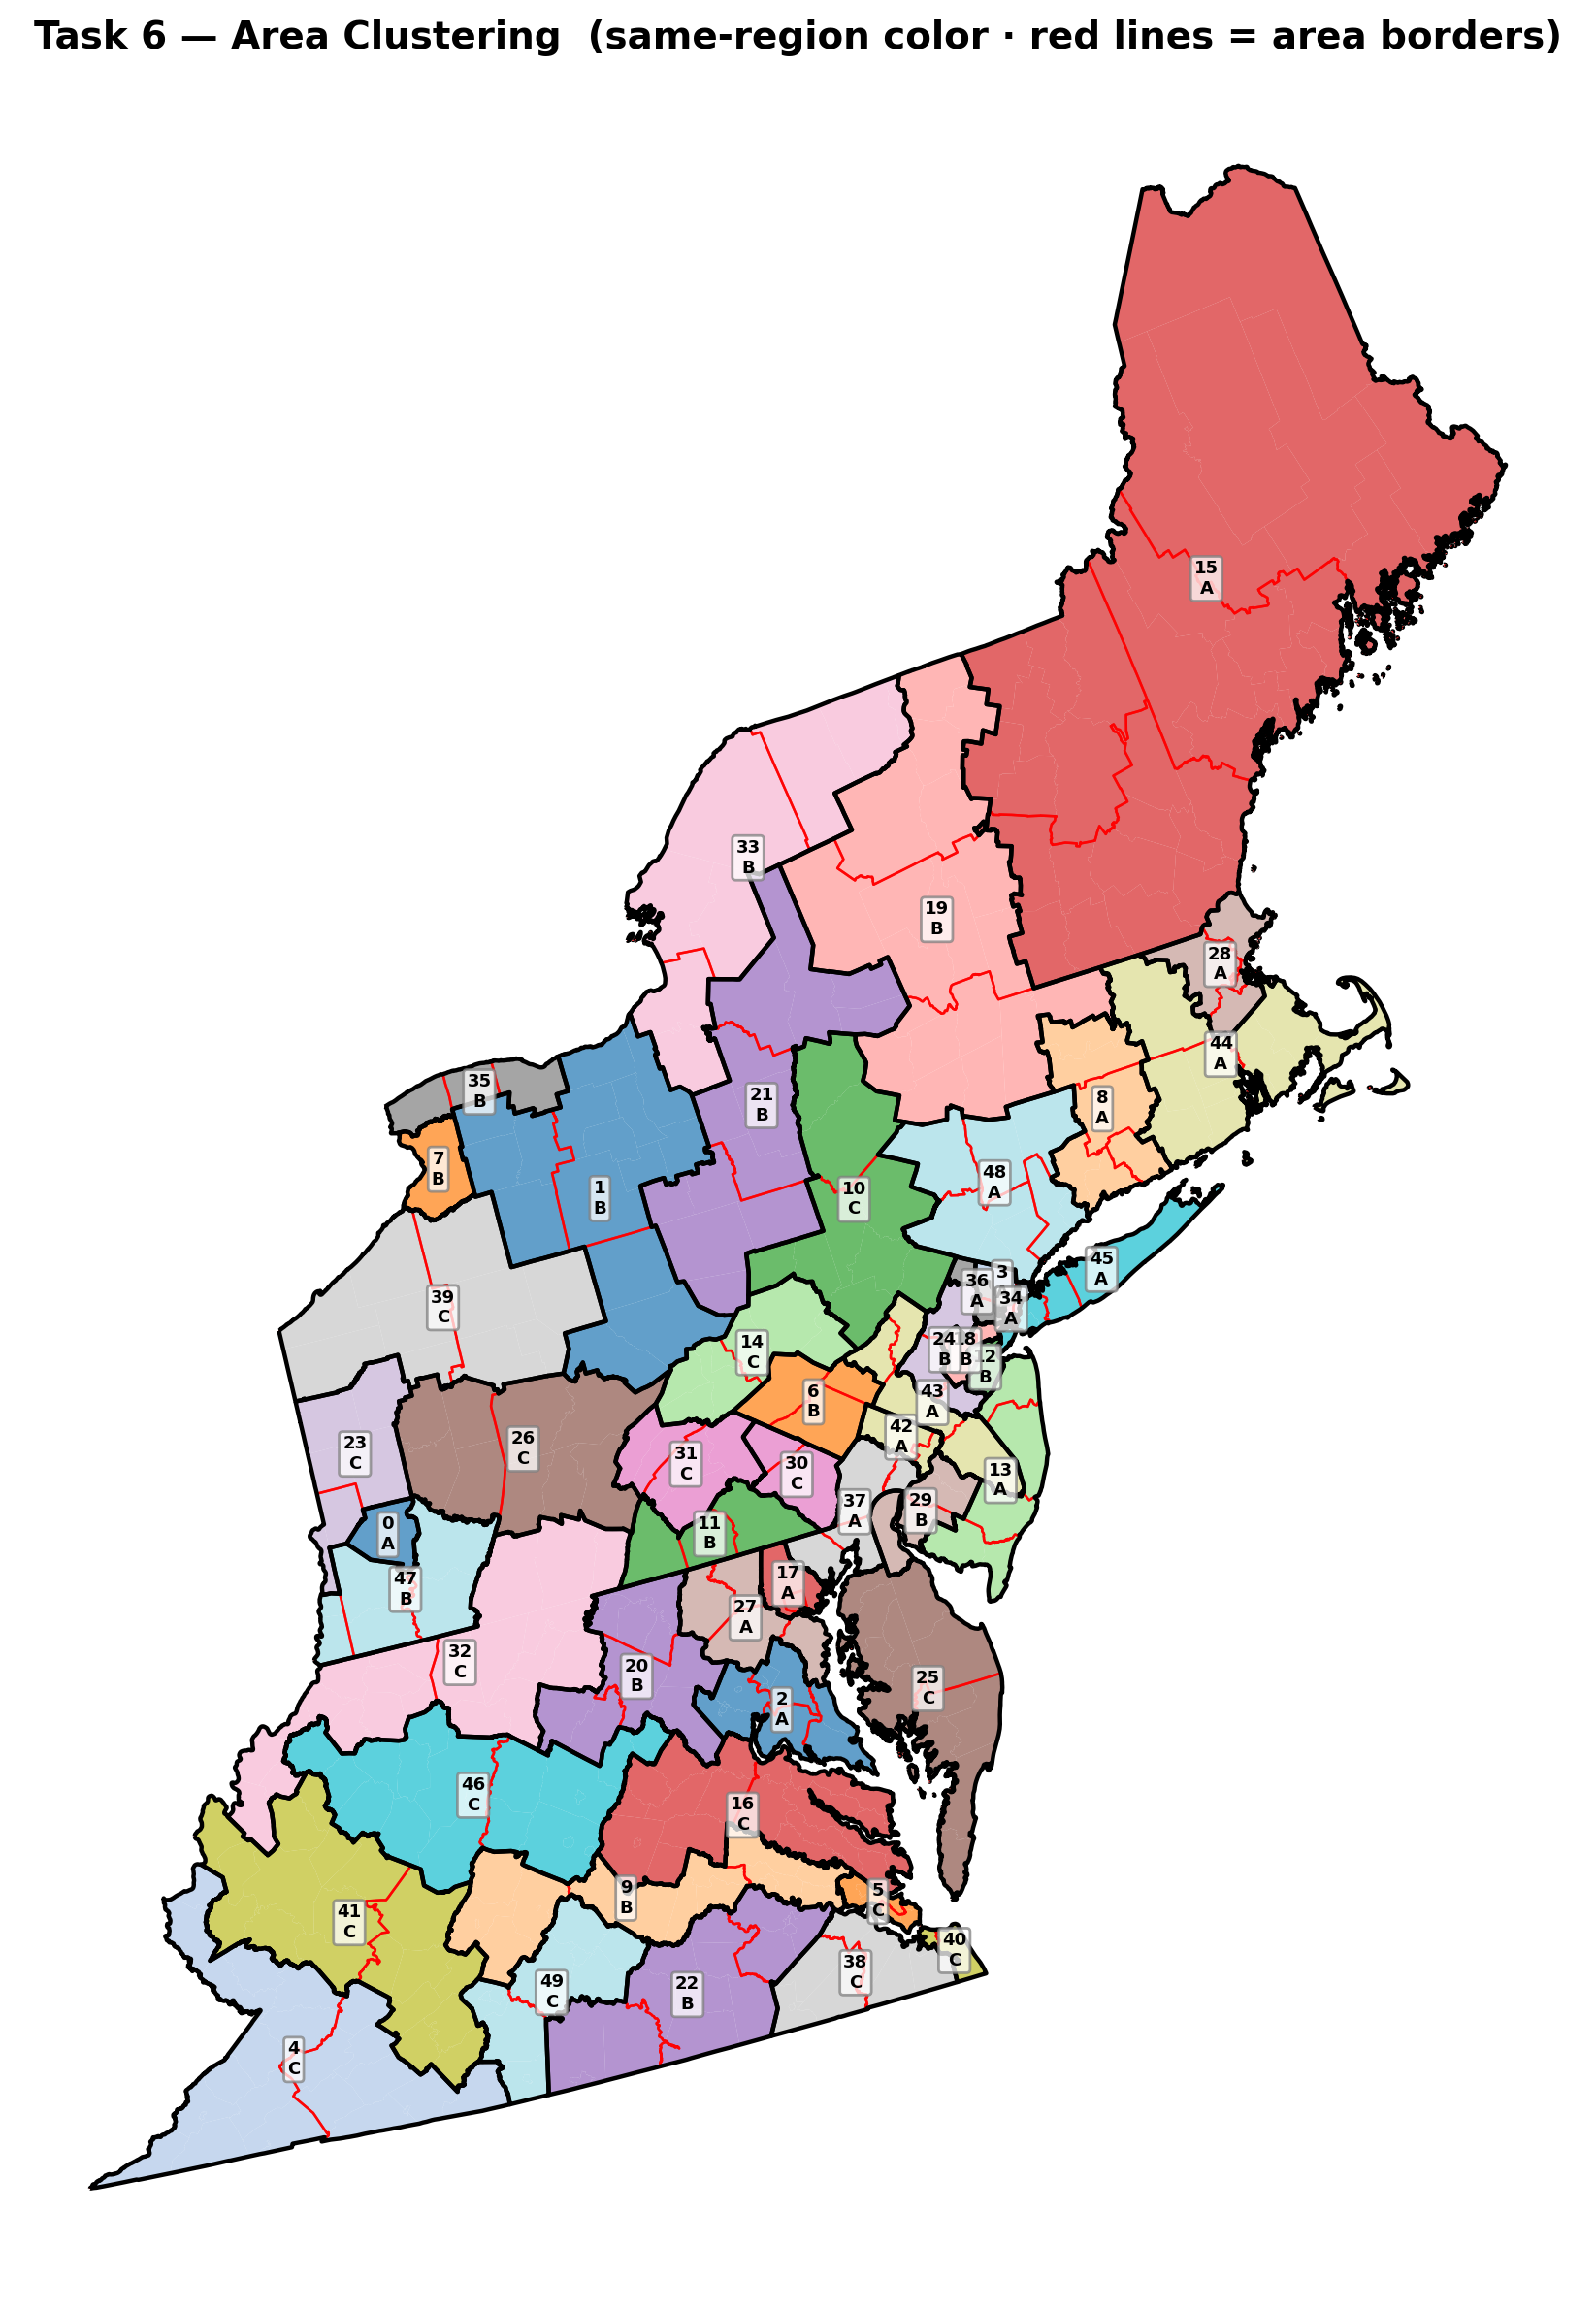
\includegraphics[width=0.90\textwidth]{figures/task6_area_map.png}
  \caption{Task~6 Phase~1 area clustering result: 132 contiguous freight areas within
    50 regions. Counties are coloured by area; thick outlines delineate Task~3 region
    boundaries. Region type (A/B/C) is labelled at each region centroid.}
  \label{fig:task6-areas}
\end{figure}

\subsection{Phase 2 — Gateway Hub Selection}

\subsubsection{Candidate Set $G$ and Feasibility Set $Z_{gw}$}

The gateway candidate pool $G$ is drawn from
\texttt{preprocessed\_capacity\_location.csv} (2,064 facilities), retaining all
facilities with usable available space $\geq 20{,}000$~sf — all 2,064 records qualify.
The 50 Task~5 regional hubs are then excluded from $G$ to prevent double-counting
facility capacity across tiers, leaving $|G| = 2{,}014$ gateway candidates.

The target gateway count per area $m_a$ is computed as:

\begin{equation}
  m_a = \max\!\left(1,\; \min\!\left(5,\;
    \left\lceil 2.0 \cdot \frac{T_a}{\bar{T}_a} \right\rceil
  \right)\right)
  \label{eq:task6-ma}
\end{equation}

where $T_a$ is the area's 2025 external throughput (ktons) and
$\bar{T}_a = 3{,}389$~ktons is the mean across all 132 areas. The distribution of
$m_a$ is: $\{1\!: 32,\; 2\!: 45,\; 3\!: 32,\; 4\!: 14,\; 5\!: 9\}$,
summing to $\Sigma m_a = 319$ gateway slots (mean 2.42 per area).

Feasible gateway–area pairs $(g, a) \in Z_{gw}$ are defined by a 50-mile Euclidean
radius from the area centroid, supplemented by in-area inclusion (any candidate whose
home county belongs to area $a$ is always included). This yields $|Z_{gw}| = 17{,}156$
feasible pairs.

\subsubsection{MIP Formulation}

The gateway MIP shares the same structural form as Task~5.
Binary variables $A_{ga} \in \{0,1\}$ indicate assignment of gateway $g$ to area $a$;
$O_g \in \{0,1\}$ indicates opening. The median candidate capacity
$\bar{Q}_{gw} = 296{,}862$~sf serves as the capacity reference.
The cost coefficient mirrors Equation~\eqref{eq:task5-cost} with area-level weights.
The constraints are:

\begin{align}
  \sum_{g:\,(g,a)\in Z_{gw}} A_{ga} &\geq m_a
    && \forall a \in A
    & \text{(coverage)} \\[4pt]
  \sum_{a:\,(g,a)\in Z_{gw}} A_{ga} &\leq 2
    && \forall g \in G
    & \text{(concentration cap)} \\[4pt]
  \sum_{g:\,(g,a)\in Z_{gw}} A_{ga} \cdot s_g &\geq \bar{Q}_{gw} \cdot \frac{T_a}{\bar{T}_a}
    && \forall a \in A
    & \text{(capacity)} \\[4pt]
  A_{ga} + A_{g'a} &\leq 1
    && \forall (g,g',a) \in S
    & \text{(separation)} \label{eq:t6-sep}
\end{align}

Constraint~\eqref{eq:t6-sep} is a key addition absent from Task~5: any two gateways
assigned to the same area must be at least 20~miles apart, preventing clustering of
hubs within a single area that would leave sub-areas unserved. The separation clash
set $S$ contains 543{,}711 triples; because $|S| > 500{,}000$, these constraints are
added lazily via a Gurobi callback on integer solutions rather than upfront, keeping
initial model build time manageable.

\subsubsection{Solution and Gateway Characterisation}

The MIP is solved to within the 1\% gap target. All 132 areas achieve full coverage
($m_a$ or more gateways assigned) with zero capacity-slack violations (minimum positive
slack: 72{,}809~sf). Table~\ref{tab:task6-results} summarises the outcome.

\begin{table}[H]
  \centering
  \caption{Task~6 Phase~2 MIP solution summary.}
  \label{tab:task6-results}
  \begin{tabular}{lr}
    \toprule
    Metric & Value \\
    \midrule
    Selected gateways & 312 \\
    Gateway-area assignments & 319 \\
    Gateways serving 1 area & 305 \\
    Gateways serving 2 areas & \phantom{0}7 \\
    Areas with negative capacity slack & 0 \\
    Min / median capacity slack (sf) & 72{,}809 / 497{,}833 \\
    \midrule
    Median gateway capacity & 350{,}381~sf \\
    Mean gateway capacity & 351{,}203~sf \\
    Min / max gateway capacity & 185{,}432 / 500{,}000~sf \\
    \bottomrule
  \end{tabular}
\end{table}

Table~\ref{tab:task6-state} shows the state distribution of the 312 selected gateways.

\begin{table}[H]
  \centering
  \caption{Selected gateway count by state.}
  \label{tab:task6-state}
  \begin{tabular}{lr}
    \toprule
    State & Gateways \\
    \midrule
    PA & 83 \\
    VA & 56 \\
    NY & 54 \\
    NJ & 43 \\
    MD & 24 \\
    MA & 15 \\
    WV & 12 \\
    CT & \phantom{0}8 \\
    DE & \phantom{0}7 \\
    ME & \phantom{0}3 \\
    NH & \phantom{0}3 \\
    RI & \phantom{0}2 \\
    VT & \phantom{0}2 \\
    \midrule
    \textbf{Total} & \textbf{312} \\
    \bottomrule
  \end{tabular}
\end{table}

By region type, gateway assignments break down as: 117 in Type~A (urban), 97 in Type~B
(suburban), and 100 in Type~C (rural). The near-parity of Type~B and Type~C counts
reflects the lower per-area demand in rural regions and the lower $m_a$ targets that
result from Equation~\eqref{eq:task6-ma}.

Figure~\ref{fig:task6-gw-locs} maps all 312 selected gateways overlaid on the regional
hub layer.

\begin{figure}[H]
  \centering
  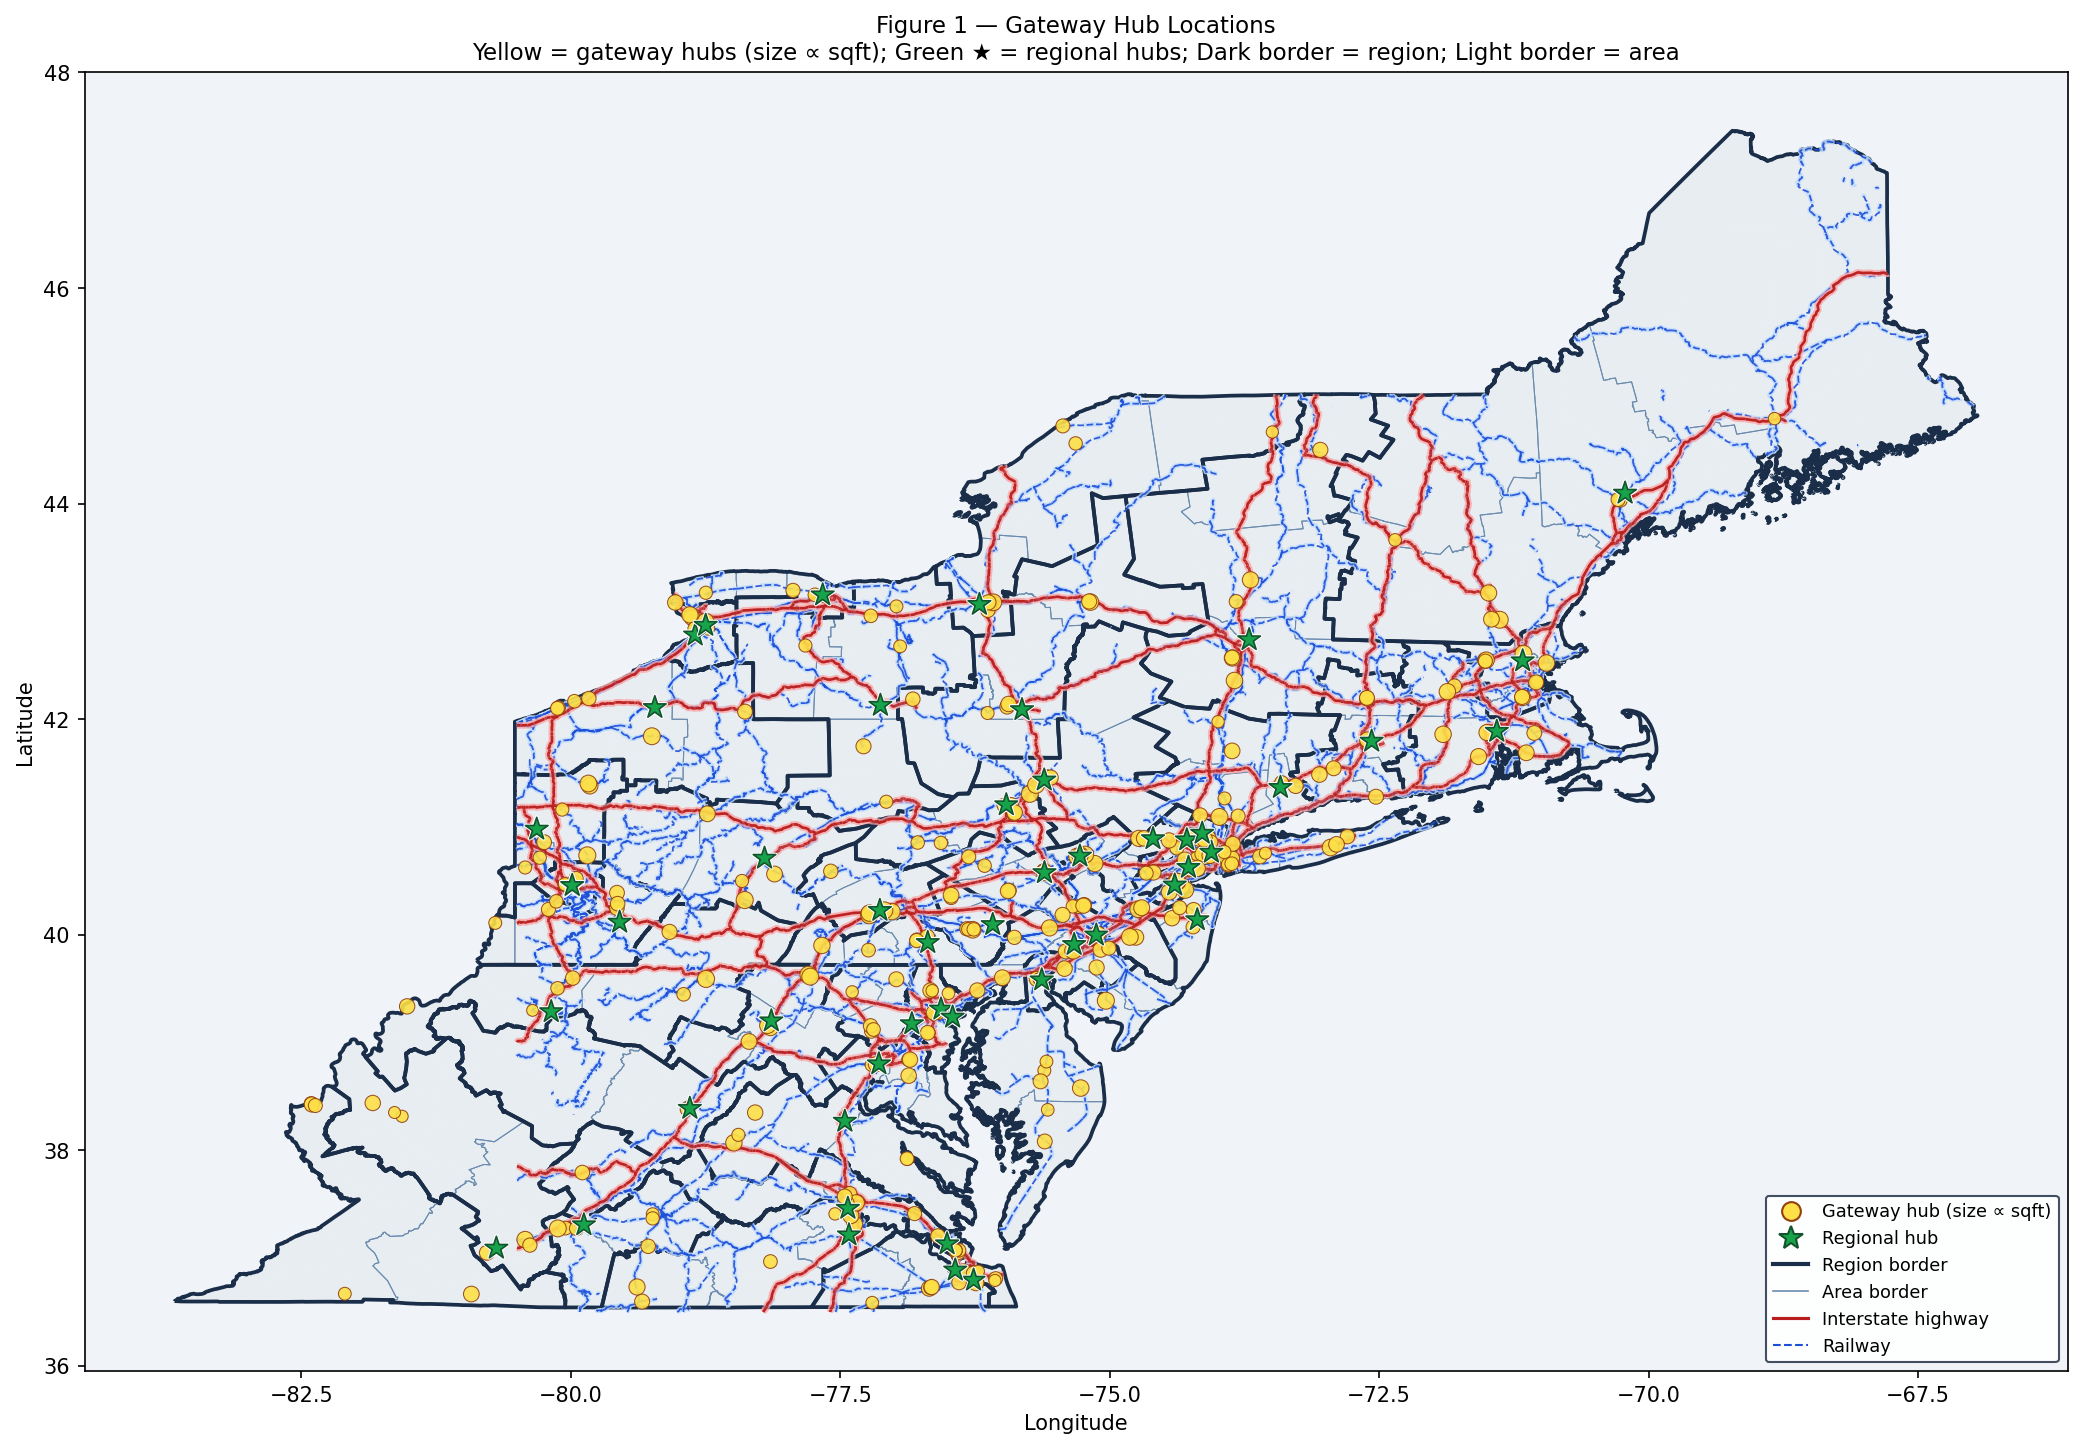
\includegraphics[width=0.90\textwidth]{figures/task6_gateway_locations.png}
  \caption{Selected gateway hubs (yellow) and regional hubs (green) across the Northeast
    megaregion. Marker size is proportional to usable available floor area. Gateways
    concentrate in the same logistics corridors as regional hubs but at finer geographic
    granularity, providing last-mile consolidation access for each freight area.}
  \label{fig:task6-gw-locs}
\end{figure}

\subsection{Network Link Definition}

Two link types are defined for the gateway tier:

\paragraph{Area-to-hub links.}
Each selected gateway is connected to the regional hub(s) assigned to its parent region.
Link attributes include distance (miles) and the area's external throughput as a flow
weight. The 132 areas generate \textbf{329 area-to-hub links} (some areas connect to
two regional hubs due to the dual assignments from Task~5). Every area has at least one
upward link, ensuring no orphaned areas in the multi-tier hierarchy.

\paragraph{Inter-area links.}
Areas within the same region that share a county border (rook adjacency, using the
Task~3 county edge table) are connected by a lateral inter-area link. This yields
\textbf{93 inter-area links}, supporting intra-region freight consolidation and
providing alternate routing paths between neighbouring areas. Link weights encode the
aggregate cross-area external throughput flow.

Figure~\ref{fig:task6-gw-network} shows the full gateway network with both link types.

\begin{figure}[H]
  \centering
  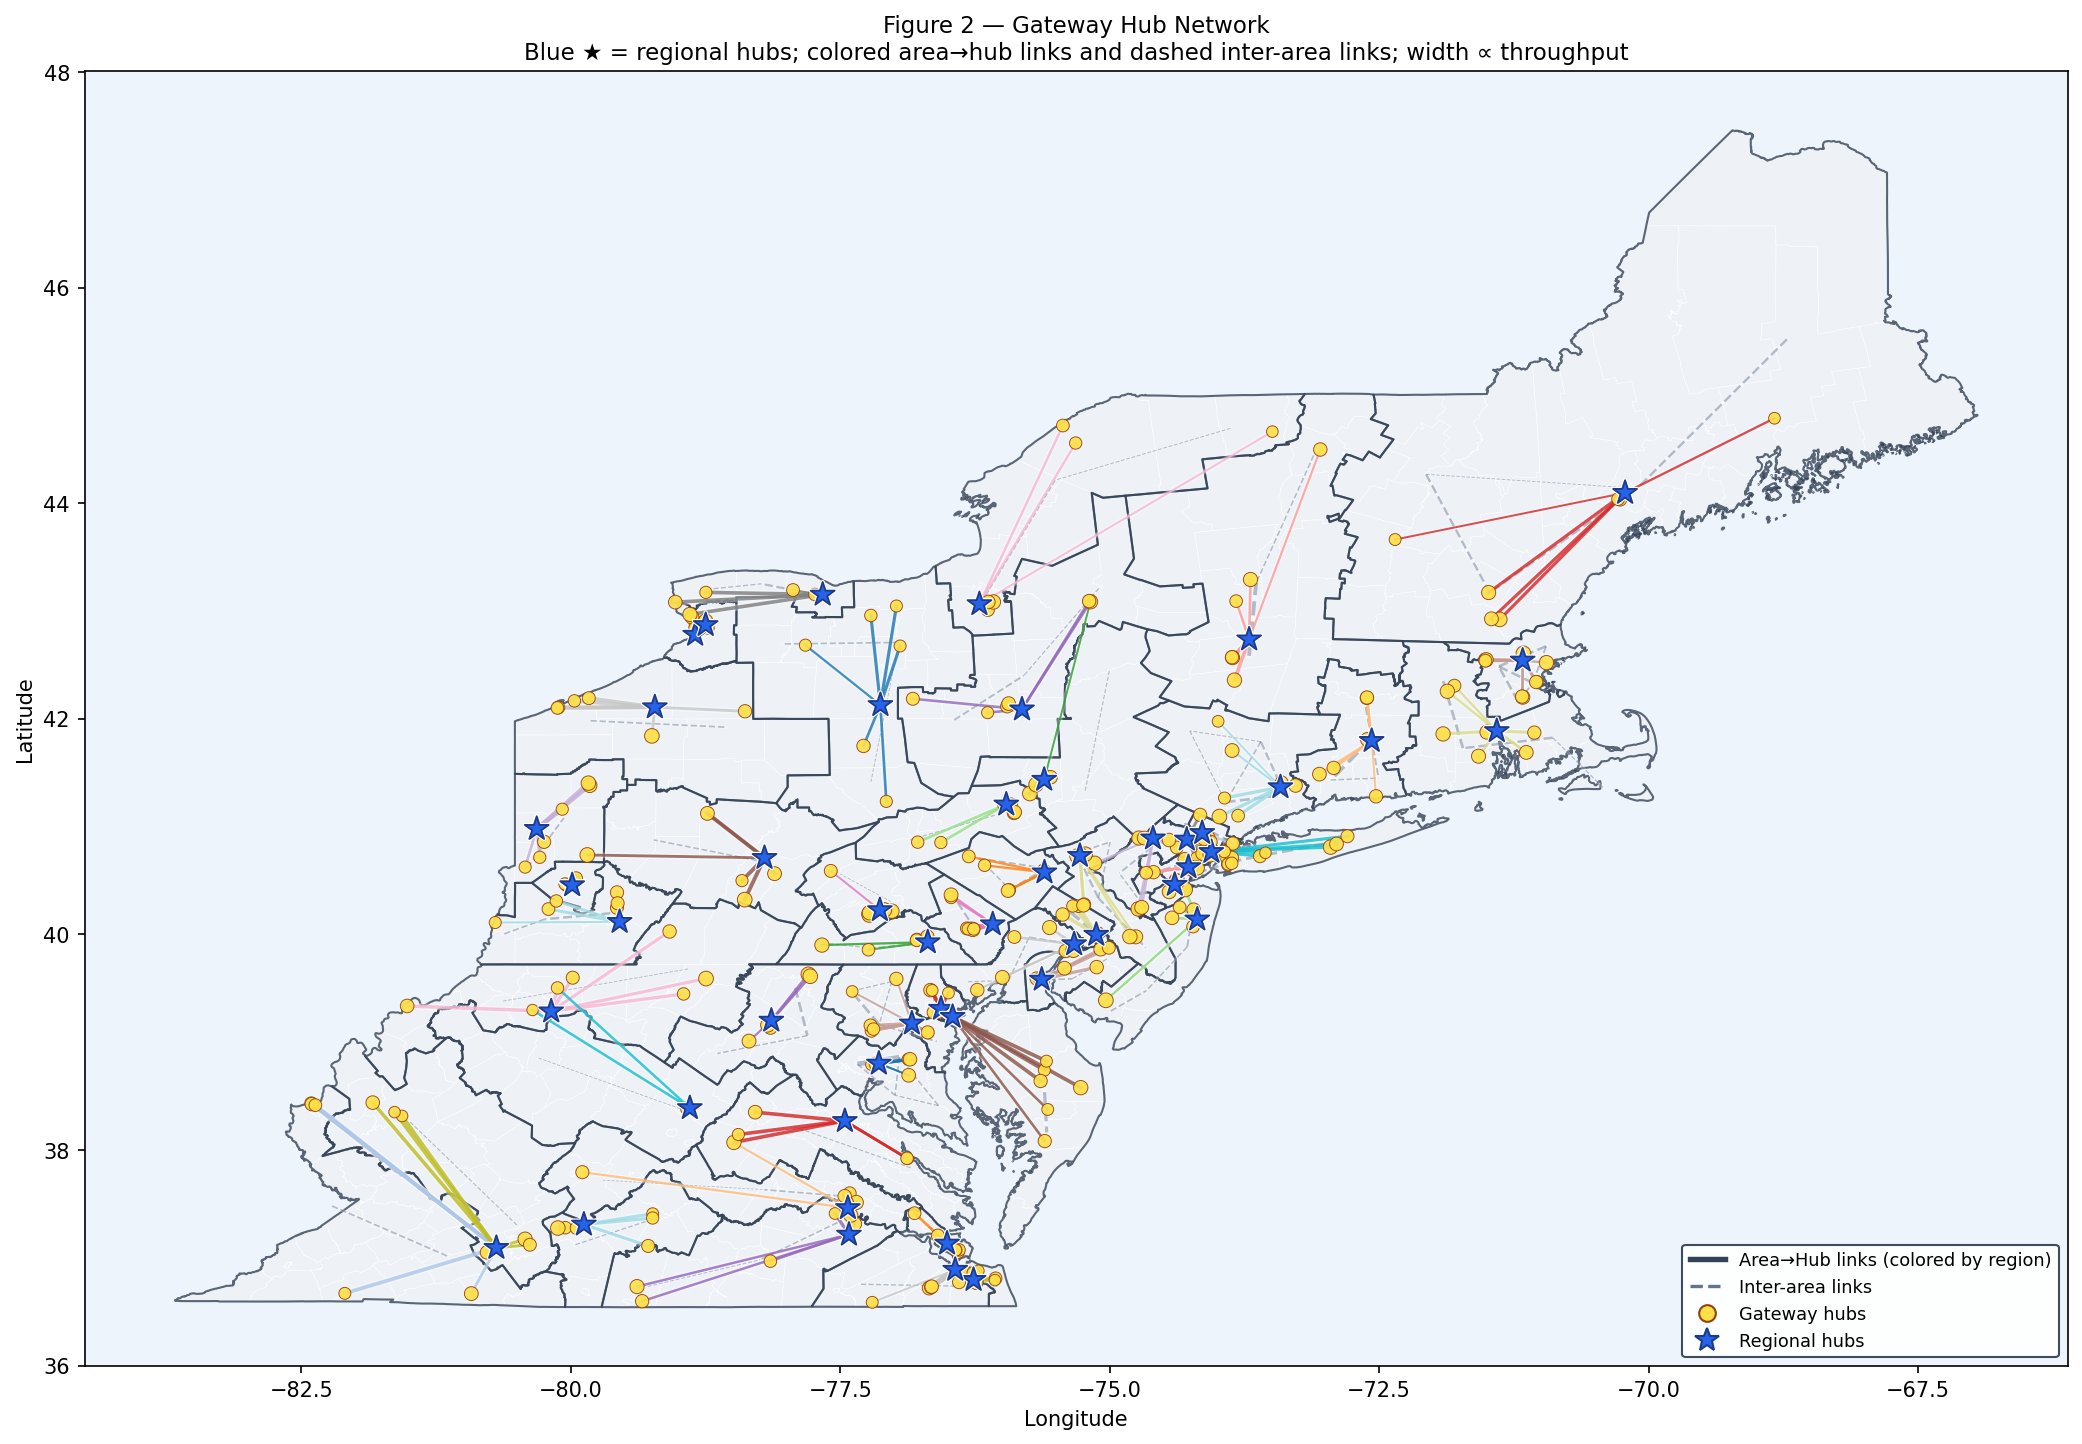
\includegraphics[width=0.90\textwidth]{figures/task6_gateway_network.png}
  \caption{Gateway hub network: area-to-regional-hub links (solid, thickness
    $\propto$ area throughput), inter-area links (dashed), gateway hubs (yellow),
    and regional hubs (blue). The dual-tier link structure connects each area both
    upward to its regional consolidation point and laterally to adjacent areas within
    the same region.}
  \label{fig:task6-gw-network}
\end{figure}
